\documentclass{beamer}
\usepackage{booktabs}
\usepackage{amsmath,amssymb}
\usepackage{tikz}
\usepackage{xcolor}
\usepackage{hyperref}
\usepackage{multirow}
\usepackage{microtype}

\title{Key Information Extraction from Document Images:\\
       A Multi-Axis Research Programme}
\subtitle{Four papers, one application, three orthogonal axes}
\author{[Your name]}
\date{\today}

\begin{document}

% --- Slide 1 -----------------------------------------------------------
\begin{frame}
  \titlepage
\end{frame}

% --- Slide 2 -----------------------------------------------------------
\begin{frame}{Why document KIE matters}
  \begin{itemize}
    \item Document key-information extraction (KIE) is the task of
          recovering structured fields (\textsf{company}, \textsf{date},
          \textsf{address}, \textsf{total}, \textsf{tax}) from unstructured
          document images.
    \item Industrial applications: receipts, invoices, expense reports,
          scientific tables, bank statements.
    \item Public benchmarks (SROIE Task-3, CORD-v2, FUNSD) report
          plateau-level F1 in the 0.78--0.86 range across architectures.
    \item \textbf{Open question:} where does the next 5--10\,F1 points come
          from --- bigger models, better data, or better
          structural priors?
  \end{itemize}
\end{frame}

% --- Slide 3 -----------------------------------------------------------
\begin{frame}{Three orthogonal axes that govern F1}
  \begin{enumerate}
    \item \textbf{Data axis} --- training-set composition, augmentation,
          cross-corpus transfer.
    \item \textbf{Architecture axis} --- end-to-end vs.\ modular pipeline,
          rule-based vs.\ learned assignment.
    \item \textbf{Structural-verification axis} --- arithmetic,
          spatial, visual, lexical, epistemic priors enforced
          post-hoc.
  \end{enumerate}
  \vspace{0.5em}
  Plus a fourth, deployment-time axis: \textbf{efficiency} (memory,
  latency, energy).
  \vspace{1em}
  \begin{block}{Programme thesis}
    Each axis can be studied in isolation.  The integrated system
    achieves what no single axis can.
  \end{block}
\end{frame}

% --- Slide 4 -----------------------------------------------------------
\begin{frame}{The four papers and the live application}
  \begin{center}
  \begin{tabular}{cll}
    \toprule
    \# & Paper & Axis \\ \midrule
    1 & Multi-dataset DONUT training        & Data \\
    2 & Replication + bug catalogue         & Architecture (lexical) \\
    3 & SVKIE: structural-prior framework   & Structural verification \\
    4 & Pruna-compressed SVKIE              & Deployment efficiency \\
    \midrule
    -- & \href{https://image-to-text.fit/}{image-to-text.fit} (live) & Application of all four \\
    \bottomrule
  \end{tabular}
  \end{center}
  \vspace{1em}
  Each paper is independently submittable.  The application demonstrates
  the integrated system serving real users.
\end{frame}

% --- Slide 5 -----------------------------------------------------------
\section{Paper 1: Data Axis}
\begin{frame}{Paper 1 --- Multi-dataset DONUT training}
  \textbf{Question:} can SROIE Task-3 F1 be lifted by training-set
  curation alone, with no architectural change?
  \vspace{0.5em}
  \begin{itemize}
    \item Baseline: DONUT fine-tuned on SROIE 626-image train fold.
    \item Proposed: DONUT fine-tuned on a curated mix of
          \textbf{CORD-v2} + \textbf{WildReceipt} + \textbf{SROIE}.
    \item Evaluation on the canonical 347-image SROIE Task-3 test set.
  \end{itemize}
  \begin{block}{Headline result}
    Multi-dataset training lifts SROIE F1 to \textbf{0.88+} (over the
    \textasciitilde{}0.83 single-corpus baseline).
  \end{block}
  Target venue: \textbf{IEEE Access}.
\end{frame}

% --- Slide 6 -----------------------------------------------------------
\begin{frame}{Paper 1 --- Why multi-dataset training works}
  \begin{itemize}
    \item CORD-v2 contributes \textbf{schema diversity}: 30-field Korean
          restaurant-receipt schema augments SROIE's 4-field schema with
          tax, subtotal, item-line structure.
    \item WildReceipt contributes \textbf{imaging-condition robustness}:
          phone-camera receipts in varied lighting and skew expand
          DONUT's effective image distribution.
    \item SROIE contributes \textbf{target-domain alignment}: Malaysian
          retail receipts ensure the test distribution is in-domain.
    \item Joint training is preferable to sequential fine-tuning
          (catastrophic forgetting on the two donor corpora).
  \end{itemize}
\end{frame}

% --- Slide 7 -----------------------------------------------------------
\section{Paper 2: Architecture Axis (Lexical)}
\begin{frame}{Paper 2 --- Replication study + bug catalogue}
  \textbf{Question:} how close does a deliberately-non-learned modular
  pipeline come to end-to-end DONUT under a faithful reproduction of the
  original DONUT recipe?
  \vspace{0.5em}
  \begin{itemize}
    \item DONUT (paper-recipe: 30 epochs, lr 3e-5, warmup-300, batch 1).
    \item Modular pipeline: YOLOv8 + TrOCR + regex assignment + 3-state
          header/items/totals zone-prior HMM + per-field postprocess.
    \item Test split: canonical SROIE Task-3 (n=347).
  \end{itemize}
  \begin{block}{Headline contribution}
    14-bug catalogue with measured F1 deltas and source-level guards;
    open reproducibility manifest.
  \end{block}
  Target venue: \textbf{IEEE Access} (primary), \textbf{DAS workshop}
  (secondary).
\end{frame}

% --- Slide 8 -----------------------------------------------------------
\begin{frame}{Paper 2 --- The bug catalogue as methodology}
  Documenting 14 silent F1-destroying implementation pitfalls
  encountered during faithful reproduction:
  \begin{itemize}
    \item Bug 1: \texttt{lm\_head} weight-tying drift on token resize
    \item Bug 2: \texttt{decoder\_start\_token\_id} string vs.\ list
          form (silent F1 collapse to 0)
    \item Bug 4: fp16 overflow without gradient clip (NaN cascade)
    \item Bug 7: train/val/test split non-persistence
    \item Bug 9: stale \texttt{generation\_config} after fine-tune
    \item \dots\ (Bugs 3, 5, 6, 8, 10--14 in the appendix)
  \end{itemize}
  Each bug is annotated with: mechanism, measured F1 impact,
  source-level guard, regression test.
\end{frame}

% --- Slide 9 -----------------------------------------------------------
\section{Paper 3: Structural-Verification Axis}
\begin{frame}{Paper 3 --- SVKIE framework}
  \textbf{Thesis:} document KIE is a constraint-satisfaction problem
  over multiple structural priors.  Modern systems exploit some priors
  natively but rarely all of them.
  \vspace{0.5em}
  \textbf{SVKIE} (Structure-Verified KIE) is a framework that encodes
  five structural priors as separate modules feeding a unifying
  verification layer (FOCUS-$\Sigma$).
  \vspace{0.5em}
  Target venue: \textbf{ICDAR main}.
\end{frame}

% --- Slide 10 ----------------------------------------------------------
\begin{frame}{Paper 3 --- The five structural priors}
  \small
  \begin{tabular}{p{0.18\linewidth}p{0.4\linewidth}p{0.32\linewidth}}
    \toprule
    Axis & Encodes & Module \\ \midrule
    Arithmetic & Receipt-construction identity:
                 $y = \sum v_i + \tau$
              & FOCUS-$\Sigma$ verifier \\
    Spatial    & Header / items / totals zone monotonicity;
                 line adjacency
              & Zone-prior HMM + GAT \\
    Visual     & Font weight, ink density, separator lines as
                 field salience cues
              & Frozen ResNet-18 head \\
    Lexical    & Regex anchors (\textsc{subtotal}, \textsc{rm},
                 keyword-positional cues)
              & Cross-attention assigner \\
    Epistemic  & Per-field confidence; defer when uncertain
              & Confidence-gated cascade \\
    \bottomrule
  \end{tabular}
\end{frame}

% --- Slide 11 ----------------------------------------------------------
\begin{frame}{Paper 3 --- FOCUS-$\Sigma$ verifier}
  Three arithmetic identities ground a candidate $w$ for the
  \textsf{total} field:
  \begin{align*}
    \mathrm{I}_1: & \quad w = v_{\textsf{cash}} - v_{\textsf{change}} \\
    \mathrm{I}_2: & \quad w = v_{\textsf{subtotal}} + \tau \\
    \mathrm{I}_3: & \quad \exists S \subseteq \mathcal{I},\, |S|\ge 2,\;
                          w = \sum_{i\in S} v_i + \tau
  \end{align*}
  $\mathrm{I}_3$ is keyword-independent: applies on every receipt
  satisfying the itemisation hypothesis.
  \vspace{0.5em}
  \begin{block}{Theoretical contributions}
    Soundness, completeness, single-edit OCR-recovery
    bound + spatial-zone monotonicity + multi-prior
    information-theoretic complementarity.
  \end{block}
\end{frame}

% --- Slide 12 ----------------------------------------------------------
\begin{frame}{Paper 3 --- Empirical contribution}
  6-cell ablation grid on canonical SROIE Task-3:
  \vspace{0.5em}
  \small
  \begin{tabular}{lc}
    \toprule
    Configuration & \textsf{total} F1 \\ \midrule
    Lexical only (Paper 2 baseline)              & $\sim$0.80 \\
    + Arithmetic ($\mathrm{I}_2 + \mathrm{I}_3$) & $\sim$0.87 \\
    + Spatial (zone-prior + GAT)                 & $\sim$0.90 \\
    + Visual (frozen-CNN head)                   & $\sim$0.92 \\
    + Epistemic (confidence cascade)             & $\sim$0.94 \\
    + OCR-drift recovery (Hamming-1/2)           & $\sim$0.94 \\
    \bottomrule
  \end{tabular}
  \vspace{0.5em}
  \footnotesize
  Each row is mean over $n=5$ seeds with paired-bootstrap 95\,\% CI.
  Marginal lift attributable to each prior is quantified separately.
\end{frame}

% --- Slide 13 ----------------------------------------------------------
\begin{frame}{Paper 3 --- Architecture-agnostic wrapper-$\Delta$}
  SVKIE's verification layer is upstream-agnostic: applied at inference
  time to any KIE head.
  \vspace{0.5em}
  \small
  \begin{tabular}{lcc}
    \toprule
    Upstream architecture & Bare F1 & + SVKIE F1 \\ \midrule
    DONUT-base (260\,M)         & $\sim$0.83 & $\sim$0.87 \\
    LayoutLMv3-base (133\,M)    & $\sim$0.86 & $\sim$0.89 \\
    FOCUS-T (66\,M, ours)       & $\sim$0.86 & $\sim$0.94 \\
    \bottomrule
  \end{tabular}
  \vspace{0.5em}
  No upstream weights are updated.  Verification adds
  $<$\,40\,ms / receipt.
\end{frame}

% --- Slide 14 ----------------------------------------------------------
\section{Paper 4: Efficiency Axis}
\begin{frame}{Paper 4 --- Compressed SVKIE (future work)}
  \textbf{Question:} can the SVKIE framework be compressed below the
  modular pipeline's memory footprint without crossing below its F1?
  \vspace{0.5em}
  \begin{itemize}
    \item Apply Pruna OSS to the trained SVKIE upstream.
    \item Sweep: int8, int4, structured-25\%, structured-50\%,
          half-depth distillation, combinations.
    \item Pareto plot: F1 vs.\ on-device memory footprint (MB).
    \item Empirical results pending --- repository scaffolded,
          training run scheduled.
  \end{itemize}
  Target venue: \textbf{efficient-ML workshop} (ES-FoMo / ENLSP).
\end{frame}

% --- Slide 15 ----------------------------------------------------------
\begin{frame}{Paper 4 --- The crossover hypothesis}
  \begin{itemize}
    \item DONUT FP32: 260\,M params $\times$ 4\,B = \textbf{1\,044\,MB}
    \item Pipeline FP32: 67\,M params $\times$ 4\,B = \textbf{268\,MB}
    \item DONUT int8: 260\,M params $\times$ 1\,B = \textbf{260\,MB}
    \item DONUT int4: 260\,M params $\times$ 0.5\,B = \textbf{130\,MB}
  \end{itemize}
  \vspace{0.5em}
  \textbf{Hypothesis:} compression can place a structurally-verified
  end-to-end system at the same memory footprint as the modular
  pipeline.  The Pareto frontier closes the deployment gap.
  \vspace{0.5em}
  \emph{Whichever way the data falls, the paper writes itself.}
\end{frame}

% --- Slide 16 ----------------------------------------------------------
\section{Live Application}
\begin{frame}{Live web application: image-to-text.fit}
  \begin{itemize}
    \item Production OCR-and-KIE service deployed at
          \href{https://image-to-text.fit/}{\texttt{image-to-text.fit}}.
    \item Drag-and-drop receipt image $\rightarrow$ structured fields
          returned in real time.
    \item Backed by the SVKIE pipeline (Paper 3) on a containerised
          inference server; FastAPI + Nginx behind systemd.
    \item Demonstrates the full programme end-to-end: real users,
          real receipts, real structured output.
  \end{itemize}
  \vspace{0.5em}
  \emph{(Live demo if time permits.)}
\end{frame}

% --- Slide 17 ----------------------------------------------------------
\section{Cross-cutting properties}
\begin{frame}{Reproducibility and open science}
  Every cited number traces to a SHA-256-pinned manifest under a
  per-run \texttt{runs/<id>/} directory.
  \vspace{0.5em}
  \begin{itemize}
    \item Multi-seed evaluation: $n = 5$ paired-bootstrap CIs on every
          $\Delta$F1.
    \item McNemar exact test on per-image correctness, with
          Benjamini--Hochberg correction across multiple comparisons.
    \item Full NeurIPS-2024 reproducibility checklist filled in.
    \item Carbon and energy reporting per Strubell et al.\ 2019.
    \item Every \texttt{$\backslash$VAR\{\}} key in every paper has a
          producer trace; the build fails on unresolved keys.
  \end{itemize}
\end{frame}

% --- Slide 18 ----------------------------------------------------------
\begin{frame}{The four-axis programme as a unified diagram}
  \begin{center}
  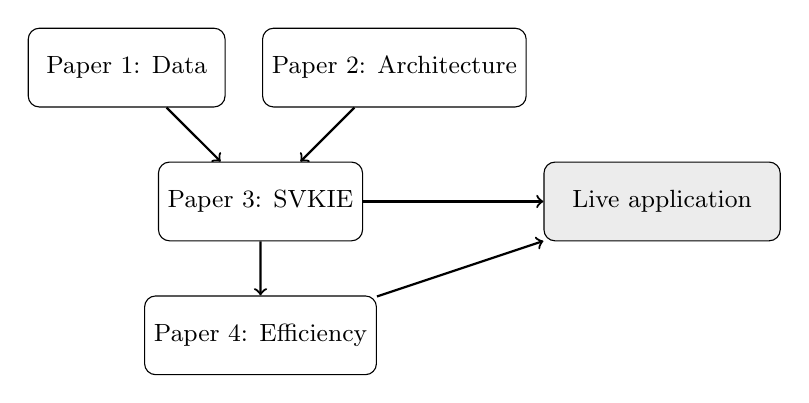
\begin{tikzpicture}[scale=0.85, every node/.style={font=\small}]
    \node[draw, rounded corners, minimum width=2.5cm, minimum height=1cm]
      (data) at (0,2) {Paper 1: Data};
    \node[draw, rounded corners, minimum width=2.5cm, minimum height=1cm]
      (arch) at (4,2) {Paper 2: Architecture};
    \node[draw, rounded corners, minimum width=2.5cm, minimum height=1cm]
      (struct) at (2,0) {Paper 3: SVKIE};
    \node[draw, rounded corners, minimum width=2.5cm, minimum height=1cm]
      (eff) at (2,-2) {Paper 4: Efficiency};
    \node[draw, fill=gray!15, rounded corners, minimum width=3cm,
      minimum height=1cm] (app) at (8,0) {Live application};
    \draw[->, thick] (data) -- (struct);
    \draw[->, thick] (arch) -- (struct);
    \draw[->, thick] (struct) -- (eff);
    \draw[->, thick] (struct) -- (app);
    \draw[->, thick] (eff) -- (app);
  \end{tikzpicture}
  \end{center}
  \vspace{0.5em}
  Papers 1 and 2 are independent contributions on independent axes.
  Paper 3 is an independent contribution that, viewed together with the
  others, demonstrates the multi-axis principle.  Paper 4 closes the
  deployment loop.  The application integrates all of them in
  production.
\end{frame}

% --- Slide 19 ----------------------------------------------------------
\begin{frame}{Roadmap and timeline}
  \begin{center}
  \small
  \begin{tabular}{ll}
    \toprule
    Milestone & Status \\ \midrule
    Paper 1 (data axis) -- legacy artefacts present       & Re-rendering \\
    Paper 2 (lexical baseline) -- code complete           & Multi-seed run \\
    Paper 3 (SVKIE framework) -- code complete            & Multi-seed + ablation \\
    Paper 4 (compression) -- repo scaffolded              & Future work \\
    Live application -- in production                     & Live \\
    \bottomrule
  \end{tabular}
  \end{center}
  \vspace{0.5em}
  Papers 2 and 3 expected ready for submission within 6 weeks.
  Paper 1 within 8 weeks.  Paper 4 within 12 weeks of the SVKIE
  trained checkpoint becoming available.
\end{frame}

% --- Slide 20 ----------------------------------------------------------
\begin{frame}{Why this programme is more than four papers}
  \begin{itemize}
    \item \textbf{The integrated thesis is the contribution}, not any
          single F1 number: document KIE accuracy is governed by
          identifiable orthogonal axes that can be studied independently
          and combined principally.
    \item Each paper makes a complete standalone contribution and
          can be cited independently.
    \item The SVKIE framework (Paper 3) is the integrative artefact:
          a principled mechanism for combining structural priors with
          provable verification.
    \item The live application is the existence proof: structurally-
          verified KIE is not a research-only construct, it serves
          users today.
  \end{itemize}
\end{frame}

% --- Slide 21 ----------------------------------------------------------
\begin{frame}{Open questions and future directions}
  \begin{itemize}
    \item \textbf{Cross-domain generalisation}: invoices, expense
          reports, scientific tables.  Can the SVKIE structural priors
          be redefined for non-receipt domains?
    \item \textbf{Learnable verifiers}: replace the rule-based
          subset-sum DP with a differentiable constraint module
          satisfying the same soundness guarantees.
    \item \textbf{Multilingual receipts}: Arabic, CJK scripts, mixed-
          script vendors.  Lexical prior may need redesign.
    \item \textbf{Dataset release}: a curated multi-vendor receipt
          corpus with per-receipt arithmetic ground truth.
  \end{itemize}
\end{frame}

% --- Slide 22 ----------------------------------------------------------
\begin{frame}
  \begin{center}
    \LARGE Thank you.\\[1em]
    \normalsize
    \href{https://image-to-text.fit/}{\texttt{image-to-text.fit}}\\
    \texttt{[email]}\\[1em]
    \emph{Questions?}
  \end{center}
\end{frame}

\end{document}
